\begin{flushright} {\tiny {\color{gray} python\_codes/fieldstone\_125/text.tex}} \end{flushright}

%\lstinputlisting[language=bash,basicstyle=\small]{python_codes/fieldstone_125/keywords}

\begin{center}

\fbox{\textbf{\huge \color{teal} P}}
Code at \url{https://github.com/cedrict/fieldstone/tree/master/python_codes/fieldstone_125}
\end{center}

\par\noindent\rule{\textwidth}{0.4pt}

%--------------------------------------------------------------------------------------------

To quote Wikipedia\footnote{\url{https://en.wikipedia.org/wiki/Voronoi_diagram}}:
``In mathematics, a Voronoi diagram is a partition of a plane into regions close to each of a given set of objects. 
In the simplest case, these objects are just finitely many points in the plane (called seeds, sites, or generators). 
For each seed there is a corresponding region, called a Voronoi cell, consisting of all points of the plane closer to 
that seed than to any other. The Voronoi diagram of a set of points is dual to its Delaunay triangulation. ''

\Literature: \textcite{may12} (2012), \textcite{hust08b} (2008).

The domain is a 2D Cartesian box. A regular grid spans this domain with resolution $nelx \times nely$. 
In each cell $nmarker\_per\_dim^2$ markers are regularly placed. 
Finally $nvo$ seeds are randomly placed in the domain and wish to compute the Voronoi cell attached to 
each seed. There are three test cases in the code, differing only by the number of seeds (7,27,111 respectively).
The are of each cell is also computed (based on the area assigned to each marker).

%-----------------------------
\subsubsection*{Test \# 1}

\begin{center}

\includegraphics[width=6cm]{python_codes/fieldstone_125/results/diagram.png}\\
{\captionfont Example with 7 seeds.}
\end{center}


%-----------------------------
\subsubsection*{Test \# 2}

\begin{center}

\includegraphics[width=6cm]{python_codes/fieldstone_125/results/test2_a}

\includegraphics[width=6cm]{python_codes/fieldstone_125/results/test2_b}\\
{\captionfont Examples with 27 random seeds.}
\end{center}

%-----------------------------
\subsubsection*{Test \# 3}

\begin{center}

\includegraphics[width=6cm]{python_codes/fieldstone_125/results/test3}
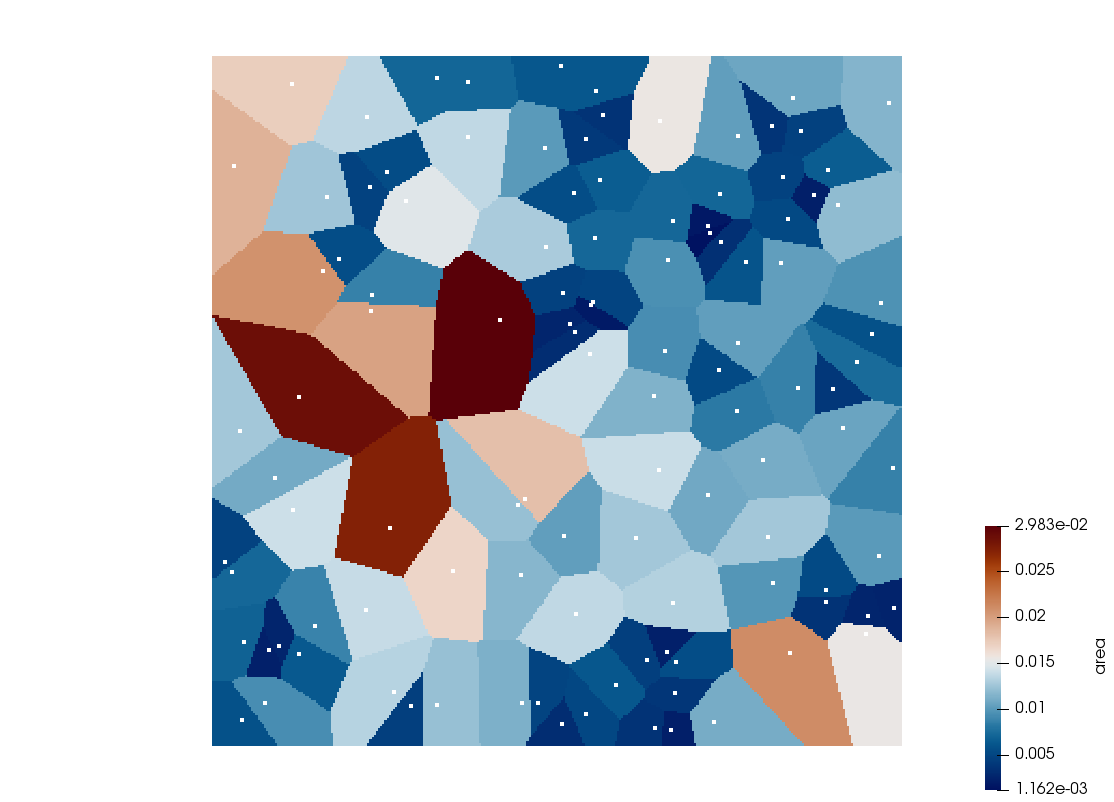
\includegraphics[width=6cm]{python_codes/fieldstone_125/results/test3_area}\\
{\captionfont Examples with 111 random seeds. Approx 310s.}
\end{center}



